\documentclass{article}
\usepackage{amssymb, amsmath, graphicx, tikz}
\usetikzlibrary{calc}
\title{Write Up\_1}
\date{}



\begin{document}

\maketitle

\textbf{1.1)} Create truth tables for X and Y and X or Y.

\vspace{3mm}

Starting with X and Y:


\begin{center}
\begin{tabular}{| c | c | c |}

X & Y & X\&Y \\
\hline
F & F & F \\
T & T & T \\
T & F & F \\
F & T & F
\end{tabular}
\end{center}

From reading the class notes,  X and Y have to be true at the same. X and Y are uniformed and are dependent on each other; if both X \& Y are true, then XY are true and same situation for X \& Y being false. When an X or  an Y is true or false, then XY are false because X \& Y are not the same. So if X is true and Y is false, then XY are false because X and Y are not the same. To help me understand this idea, I thought of pair of socks: if same pair of socks, then true (they belong together). If mismatched socks, then false (they don't go together).

\vspace{1in}

Now with X or Y:

\begin{center}
\begin{tabular}{| c | c | c |}
X & Y & X or Y \\
\hline
F & F & F \\
T & T & T \\
T & F & T \\
F & T & T
\end{tabular}
\end{center}

For this, X is independent and Y is independent. Since X and Y don't depend on each other, then X or Y is true when either a X is true, a Y is true, or X and Y is true. I took CS161 class and we basically used the same idea. This is what we did:




\includegraphics[width=0.9\columnwidth]{../Desktop/IMG_0516.HEIC.pdf}


Reference: CS161 Notes


\vspace{3mm}

Explanation: What we did was we were trying to figure out what the print statement would be if we input a number that was 
$\ge18$ and/or $\le35$. We did a truth table to help us understand that. 

\newpage


\textbf{1.2)}  Consider the following statement, for which n represents an unknown integer: If $n<5$, then $n<10.$

\vspace{3mm}

Referring back to the definition from class notes:

\vspace{3mm}

\begin{center}
Definition of Negation: If X, then $\sim$Y\\

\hspace{.09mm}Definition of Converse: If Y, then X\\


\hspace{.4in} Definition of Contrapositive: If $\sim$Y, then $\sim$X\\


Definition of Inverse: If $\sim$X, then $\sim$Y. 

\end{center}

\vspace{3mm}


\textbf{Form of statement:}
\vspace{3mm}


Negation: If n$<$5, then n$>$10

\vspace{2mm}

Converse: If n$<$10, then n$<$5

\vspace{2mm}

Contrapositive: If n$>$10, then n$>$5

\vspace{2mm}

Inverse: If n$>$5, then n$>$10

\vspace{3mm} 

\textbf{i)} I don't think any of these forms of the conditional statement are true for any n. 

For converse: if n=2, then it would be less than 10 and 5. It says that \textbf{n is any integer}, so if n=6, then it wouldn't be less than 5, and therefore this would be false.
\vspace{2mm}

For contrapositive: if n =2, this would make this form of the conditional statement false.
\vspace{2mm}

For inverse: same idea as contrapositive.
\vspace{2mm}

For Negation: this won't work either.

\vspace{3mm}

\textbf{ii)} Negation, because if the $n<5$ and $n>10$ are working against each other. If we chose one n, then it would make this statement false.

\vspace{3mm} 

\textbf{iii)} Making drawings for this would help me understand what is going on:

\vspace{3mm}

For Negation: 
\begin{center}
\begin{tabular}{| c | c | c |}

$n <5$ & $n>10$ &  $X \rightarrow \sim$Y \\
\hline
F & F & T\\
T & T & F \\
T & F & T \\
F & T & T
\end{tabular}
\end{center}



For Converse: 
\begin{center}
\begin{tabular}{| c | c | c |}

$n<10$ & $n<5$ & Y $\rightarrow$ X \\
\hline
F & F & F \\
T & T & T \\
T & F & T\\
F & T & F
\end{tabular}
\end{center}

For contrapostive: 

\begin{center}
\begin{tabular}{| c | c | c |}

$n >10$ & $n>5$ & $\sim Y \rightarrow \sim X$ \\
\hline
F & F & F \\
T & T & T \\
T & F & F \\
F & T & T
\end{tabular}
\end{center}

\vspace{3mm} 

For inverse: 
\begin{center}
\begin{tabular}{| c | c | c |}

$n >5$ & $n>10$ & $\sim X \rightarrow \sim $ Y \\
\hline
F & F & F \\
T & T & T \\
T & F & T \\
F & T & F
\end{tabular}
\end{center}
\vspace{3mm}
After figuring out how the table would result for each on scrap paper, I came to the conclusion that converse and inverse were logically equivalent. 

I processed like this on my scrap paper: If there was an integer that was both greater than 10 (T), then the integer is definitely be greater than 5 (T) which makes this true. If the integer was less than 10 (F), then less then 5 (F), which makes this false. We would proceed this with idea with the rest of the tables. For the all the false and true (first and second columns), I thought of its' opposites: if $n>5$ was false, then I would think that $n<5$ and same idea with the trues. While doing this, I would then got the results for the third column. 

\newpage
\textbf{1.4a)} Consider the following statements, for which A, B, and C represent distinct points: 

\vspace{3mm}

X is the statement "A and B are collinear."

Y is the statement "B is between A and C."
\vspace{3mm}

Making a drawing:

\begin{center}
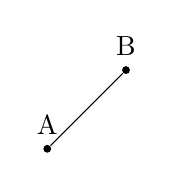
\begin{tikzpicture}[dot/.style={circle,inner sep=1pt,fill,label={#1},name=#1},
  extended line/.style={shorten =-#1,shorten =-#1},
  extended line/.default=1cm]

\node [dot=A] at (2,1) {};
\node [dot=B] at (3,2) {};
\draw [] (A) -- (B);
\end{tikzpicture}
\end{center}




\begin{center}
\begin{tikzpicture}[dot/.style={circle,inner sep=1pt,fill,label={#1},name=#1},
  extended line/.style={shorten =-#1,shorten =-#1},
  extended line/.default=1cm]
\node [dot=A] at (2,1) {};
\node [dot=B] at (3,2) {};
\node [dot=C] at (4,3) {};

\draw [] (A) (B) (C);
\end{tikzpicture}
\end{center}



Is (X and Y) true or false?:
\vspace{3mm}

I think this is false. X is saying that AB are collinear and Y is saying that ABC are collinear. AB is not the same as ABC. As I mentioned before then and would mean that X \& Y would have be the same; since it is not the, this is false. 

\vspace{1in}


\textbf{1.4b)} Is (X or Y) true or false?

\vspace{3mm}

This would be true. As stated in the class notes, the or can be inclusive or exclusive so the statements can be different. 
Since X is the statement "A and B are collinear" and Y is the statement "B is between A and C," then this is true because which they are saying different thing, but they are both true.


\newpage 

\textbf{1.4c)} Is (if X, then Y) true or false?

\vspace{3mm}

This is saying if "A and B are collinear," then "B is between A and C." I believe this is neither because there is not enough information on statement Y. One is talking about AB being collinear and the other one is talking about B is between A and C. What I don't know is if these  A, B, and C lie are on the same line. 

I came to this conclusion because I remember during our group meeting, we were debating if 1.3 was true or not. We came to the conclusion of neither because there was not enough information. 


\vspace{3mm}

\begin{center}
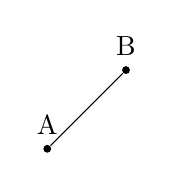
\begin{tikzpicture}[dot/.style={circle,inner sep=1pt,fill,label={#1},name=#1},
  extended line/.style={shorten =-#1,shorten =-#1},
  extended line/.default=1cm]

\node [dot=A] at (2,1) {};
\node [dot=B] at (3,2) {};
\draw [] (A) -- (B);
\end{tikzpicture}
\end{center}
 
\begin{center}
\begin{tikzpicture}[dot/.style={circle,inner sep=1pt,fill,label={#1},name=#1},
  extended line/.style={shorten =-#1,shorten =-#1},
  extended line/.default=1cm]
\node [dot=A] at (2,1) {};
\node [dot=B] at (3,2) {};
\node [dot=C] at (4,3) {};

\draw [] (A) (B) (C);

\end{tikzpicture}
\end{center}
  

\newpage 

\textbf{1.4d)} Is (if Y, then X) true or false?

\vspace{3mm}

This is saying that if "B is between A and C," then "A and B are collinear." I think this true. I basically made two drawing and added the idea together and made a 3rd drawing:


\begin{center}
\begin{tikzpicture}[dot/.style={circle,inner sep=1pt,fill,label={#1},name=#1},
  extended line/.style={shorten >=-#1,shorten <=-#1},
  extended line/.default=1cm]

\node [dot=A] at (2,1) {};
\node [dot=B] at (3,2) {};
\node [dot=C] at (4,3) {};

\draw [] (A) (B) (C);

\end{tikzpicture}
\end{center}

\begin{center}
+
\end{center}


\begin{center}
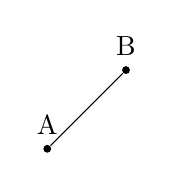
\begin{tikzpicture}[dot/.style={circle,inner sep=1pt,fill,label={#1},name=#1},
  extended line/.style={shorten =-#1,shorten =-#1},
  extended line/.default=1cm]

\node [dot=A] at (2,1) {};
\node [dot=B] at (3,2) {};
\draw [] (A) -- (B);
\end{tikzpicture}
\end{center}

\begin{center}
=
\end{center}

\begin{center}
\begin{tikzpicture}[dot/.style={circle,inner sep=1pt,fill,label={#1},name=#1},
  extended line/.style={shorten >=-#1,shorten <=-#1},
  extended line/.default=1cm]

\node [dot=A] at (2,1) {};
\node [dot=C] at (4,3) {};
\node [dot=B] at (3,2) {};

\draw [] (A) -- (B) (C);

\end{tikzpicture}
\end{center}



\end{document}
